% Payroll Management System SRS (2-3 pages)
\documentclass[11pt]{article}
\usepackage[margin=1in]{geometry}
\usepackage{array}
\usepackage{enumitem}
\usepackage{xcolor}
\usepackage{hyperref}
\usepackage{tikz}
\usepackage{float} % for [H] placement of figures
\usetikzlibrary{positioning,arrows.meta,shapes.geometric,shapes.misc}
\setlist{nosep}

\title{Software Requirements Specification}

\begin{document}

\begin{titlepage}
    \centering
    \vspace*{2.5cm}

    {\color{teal}\rule{\linewidth}{1.5pt}\par}
    \vspace{0.6cm}
    {\Huge\bfseries Payroll Management System\par}
    
    \vspace{0.6cm}
    {\color{teal}\rule{\linewidth}{1.5pt}\par}

    \vspace{1.8cm}
    {\large\itshape Streamlined payroll tracking with overtime, allowances, and exports\par}

    \vfill
    \begin{flushright}
        {\Large Yash Kumar Jain (2023UCP1571)\\[0.3cm] Dhruv Bansal (2023UCP1570)\\[0.3cm] Nakshatra Bansal (2023UCP1575)}
    \end{flushright}

    \vspace{1cm}
    {\large\today\par}
\end{titlepage}

\clearpage

\section*{Project Links \& Group Details}
\vspace{0.4cm}

\noindent\fbox{%
  \parbox{\dimexpr\linewidth-2\fboxsep-2\fboxrule}{%
    \vspace{0.4cm}
    \begin{center}
        {\Large\bfseries Project Links \& Group Details}\\[0.2cm]
        \rule{\linewidth}{0.4pt}
    \end{center}

    \vspace{0.6cm}
    {\large\textbf{Project Title:}} \hspace{0.5cm} Payroll Management System\\[0.6cm]

    {\large\textbf{Group Number:}} \hspace{0.5cm} \textbf{G-10}\\[0.6cm]
    \rule{\linewidth}{0.4pt}

    \vspace{0.6cm}
    \begin{center}
        {\large\bfseries Group Members:}
    \end{center}
    \vspace{0.3cm}
    {\large
    1.\; Yash Kumar Jain \hfill Reg. No.\ 2023UCP1571\\[0.3cm]
    2.\; Dhruv Bansal \hfill Reg. No.\ 2023UCP1570\\[0.3cm]
    3.\; Nakshatra Bansal \hfill Reg. No.\ 2023UCP1575\\[0.6cm]
    }
    \rule{\linewidth}{0.4pt}

    \vspace{0.8cm}
    \begin{center}
        {\large\bfseries GitHub Repository Link:}\\[0.2cm]
        {\large\textcolor{blue}{\href{https://github.com/thesilverwolfx/payroll\_management\_system}{https://github.com/thesilverwolfx/payroll\_management\_system}}}
    \end{center}

    \vspace{0.8cm}
    \begin{center}
        {\large\bfseries YouTube Demo Video (Unlisted):}\\[0.2cm]
        {\large\textcolor{blue}{\href{https://youtube.com/watch?v=your-demo-link}{https://youtube.com/watch?v=your-demo-link}}}
    \end{center}

    \vspace{0.2cm}
  }%
}

\clearpage

\section{Abstract}
The Payroll Management System is a lightweight web application built with Python and Flask to support small teams in managing hourly employees. 
It streamlines employee record keeping, tracks working hours, applies overtime rules, and incorporates allowances and deductions to compute gross and net pay. 
The system offers an at-a-glance payroll dashboard, CSV export for downstream processing, and robust local persistence via JSON files, making it well suited for academic and small-scale organizational use.

\section{Project Introduction}
Modern organizations require fast and reliable access to payroll information, even when operating without complex enterprise infrastructure. 
This project aims to provide a simple yet extensible payroll solution that can be deployed locally, used by a single HR operator, and adapted for future enhancements such as database backends or authentication. 
The application focuses on clarity of interface, correctness of calculations, and maintainable architecture so that students and practitioners can both operate and extend the system with ease.

\section{SRS Introduction}
\textbf{Purpose.} This Software Requirements Specification (SRS) defines the functional and non-functional requirements for the Payroll Management System so that stakeholders, developers, and reviewers share a common understanding of the release scope.

\noindent\textbf{Scope.} The SRS covers employee data management, hours and compensation updates, payroll calculation with overtime, reporting and CSV export, and local data persistence. 
It excludes tax engines, multi-user access control, and integration with external payment services.

\noindent\textbf{Definitions.} Employee ID (unique string), Overtime (hours beyond 40 weekly at 1.5$\times$ rate), Allowance (positive adjustment), Deduction (withholding), JSON (data serialization), CSV (comma-separated values export format).

\section{Overall Description}
\subsection{Product Perspective}
Standalone Python/Flask service; stores state in \texttt{payroll\_data.json}; HTML interface rendered via Jinja templates; no external database or authentication.

\subsection{User Characteristics}
Small HR/admin teams with basic payroll knowledge, single concurrent operator, working on desktop or tablet browsers.

\subsection{Assumptions and Constraints}
\begin{itemize}
    \item Trusted environment; no login or role management.
    \item File-system write access required for persistence/export.
    \item Local host deployment; internet connectivity optional (only for documentation).
    \item Target document length is 2--3 pages; functionality limited to hourly wages (no tax engine).
\end{itemize}

\section{Functional Requirements}
\subsection{FR1: Employee Records}
\textit{Description:} Create, list, and delete employee profiles with name, ID, department, hourly rate, allowances, deductions, and hours worked.\\
\textit{Rationale:} Core HR data storage.\\
\textit{Acceptance:} Unique ID enforced; data persists after restart; list view displays all fields.

\subsection{FR2: Compensation Updates}
\textit{Description:} Edit hours, allowances, or deductions simultaneously; blank inputs keep prior values.\\
\textit{Rationale:} Speeds weekly adjustments.\\
\textit{Acceptance:} Validation prevents negative values; success flash message confirms update.

\subsection{FR3: Payroll Calculation}
\textit{Description:} Compute regular/overtime hours, base pay, overtime pay, gross pay, and net pay per employee and as cumulative totals.\\
\textit{Rationale:} Provides financial visibility.\\
\textit{Acceptance:} Dashboard shows employee count, total hours, gross/net sums, average rate; payroll table refreshes automatically.

\subsection{FR4: Reporting and Export}
\textit{Description:} Render payroll tables on the dashboard and provide a CSV download with per-employee breakdown plus totals.\\
\textit{Rationale:} Enables auditing and spreadsheet workflows.\\
\textit{Acceptance:} CSV headers match on-screen metrics; download triggers from UI button.

\subsection{FR5: Data Persistence}
\textit{Description:} Auto-save after any CRUD or compensation update and reload on startup. Handle corrupted files by falling back to an empty dataset without crashing.\\
\textit{Rationale:} Prevents data loss.\\
\textit{Acceptance:} JSON file reflects latest state; application remains operable after file manipulation errors.

\section{Non-Functional Requirements}
\textbf{Usability.} Single-page layout with validated forms, flash feedback, and responsive cards that remain legible on tablets.\\
\textbf{Performance.} CRUD and payroll calculations return within one second for up to 200 employees on commodity hardware.\\
\textbf{Reliability.} Validation ensures numeric inputs, overtime logic always runs, and CSV export degrades gracefully if no employees exist.\\
\textbf{Maintainability.} Separation between Flask routes, business logic module, and templates; minimal dependencies (Flask only).\\
\textbf{Portability.} Runs on Windows/macOS/Linux with Python 3.11+ and modern browsers (Chrome, Edge, Firefox, Safari).

\section{Interface Requirements}
\textbf{User Interface.} HTML5/CSS layout with summary cards, employee table, payroll table, and forms for add/update flows; download link for CSV export.\\
\textbf{Software Interfaces.} Flask routing, local JSON storage, CSV stream for download, browser-based HTTP client.\\
\textbf{Hardware Interfaces.} None beyond a device capable of running a browser.\\
\textbf{Communication.} HTTP over localhost (default port 5000); no external API traffic.

\section{Traceability Matrix (Excerpt)}
\begin{tabular}{|>{\raggedright}p{1.5cm}|p{6cm}|p{6cm}|}
\hline
\textbf{ID} & \textbf{Requirement} & \textbf{Implementation Hook} \\
\hline
FR1 & Manage employee profiles & Flask route \texttt{/add\_employee}, persistence in \texttt{PayrollSystem.add\_employee} \\
\hline
FR2 & Update compensation inputs & Route \texttt{/update\_compensation}, \texttt{PayrollSystem.update\_compensation} \\
\hline
FR3 & Compute payroll + summary & \texttt{PayrollSystem.calculate\_payroll}, dashboard cards \\
\hline
FR4 & Export CSV & Route \texttt{/export\_payroll}, \texttt{PayrollSystem.export\_payroll\_csv} \\
\hline
FR5 & Persist data & \texttt{load\_data} and \texttt{save\_data} methods \\
\hline
\end{tabular}

\section{Risks and Mitigations}
\begin{itemize}
    \item \textbf{Corrupted JSON file} -- mitigate with try/except and empty fallback.
    \item \textbf{Incorrect manual entries} -- rely on on-field validation and flash guidance.
    \item \textbf{Future scaling needs} -- design keeps logic modular so a database backend can replace the JSON store later.
\end{itemize}

\section{Approval}
Stakeholders sign off electronically by referencing this LaTeX-formatted SRS in the project tracking system.

\clearpage

\section{UML Diagrams}
This section presents key UML views of the Payroll Management System, including use-case, class, sequence, and component diagrams. 
They collectively describe how users interact with the system, how core entities are structured, how major workflows execute over time, and how the application is decomposed into deployable parts.

\subsection{Class Diagram}
The class diagram models the main domain classes, including \texttt{Employee}, \texttt{PayrollSystem}, and supporting utility classes responsible for persistence and reporting.

\begin{figure}[H]
    \centering
    \vspace{1cm}
    \begin{tikzpicture}[
        class/.style={draw, rectangle, rounded corners,
                      minimum width=4.5cm, align=left, font=\small},
        relation/.style={-Stealth}
    ]
        % Employee
        \node[class] (Employee) at (0,0) {
            \textbf{Employee}\\\hline
            - name : string\\
            - employeeId : string\\
            - hourlyRate : float\\
            - hoursWorked : float\\
            - department : string\\
            - allowances : float\\
            - deductions : float\\\hline
            + calculatePay() : PayBreakdown\\
            + toDict() : dict
        };

        % PayrollSystem
        \node[class,right=3cm of Employee] (PS) {
            \textbf{PayrollSystem}\\\hline
            - dataFile : string\\
            - employees : dict\\
            - overtimeThreshold : float\\
            - overtimeMultiplier : float\\\hline
            + loadData() : void\\
            + saveData() : void\\
            + addEmployee() : (bool,string)\\
            + removeEmployee() : (bool,string)\\
            + updateCompensation() : (bool,string)\\
            + calculatePayroll() : (list,totals)\\
            + getSummary() : Summary\\
            + exportPayrollCsv() : string
        };

        % PayBreakdown
        \node[class,below=2.5cm of Employee] (PB) {
            \textbf{PayBreakdown}\\\hline
            + regularHours : float\\
            + overtimeHours : float\\
            + basePay : float\\
            + overtimePay : float\\
            + grossPay : float\\
            + netPay : float
        };

        % FlaskApp
        \node[class,below=2.5cm of PS] (FA) {
            \textbf{FlaskApp}\\\hline
            + index()\\
            + add\_employee()\\
            + update\_compensation()\\
            + remove\_employee()\\
            + export\_payroll()
        };

        % Relations
        \draw[relation] (PS.west) -- node[above]{manages} (Employee.east);
        \draw[relation] (FA.north) -- node[right]{uses} (PS.south);
        \draw[relation] (Employee.south) -- node[left]{returns} (PB.north);
    \end{tikzpicture}
    \caption{Class Diagram for Core Payroll Classes}
\end{figure}

\clearpage

\subsection{Component Diagram}
The component diagram summarizes the high-level architecture, separating the web UI, Flask application layer, business logic module, and local JSON/CSV storage components.

\begin{figure}[H]
    \centering
     \vspace{1cm}
    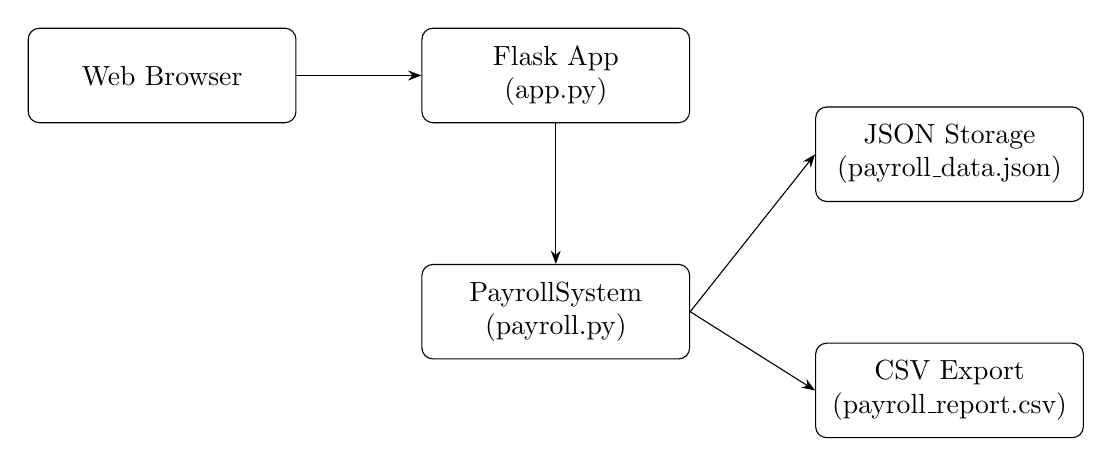
\begin{tikzpicture}[
        comp/.style={draw, rectangle, minimum width=3.4cm, minimum height=1.2cm,
                     align=center, rounded corners},
        dep/.style={-Stealth}
    ]
        \node[comp] (browser) at (0,0) {Web Browser};
        \node[comp] (flask)   at (5,0) {Flask App\\(app.py)};
        \node[comp] (logic)   at (5,-3) {PayrollSystem\\(payroll.py)};
        \node[comp] (json)    at (10,-1) {JSON Storage\\(payroll\_data.json)};
        \node[comp] (csv)     at (10,-4) {CSV Export\\(payroll\_report.csv)};

        \draw[dep] (browser.east) -- (flask.west);
        \draw[dep] (flask.south) -- (logic.north);
        \draw[dep] (logic.east) -- (json.west);
        \draw[dep] (logic.east) -- (csv.west);
    \end{tikzpicture}
    \caption{Component Diagram for Payroll Management System}
\end{figure}

\subsection{Sequence Diagram}
The sequence diagram illustrates the high-level flow when an HR user updates compensation for an employee and views the refreshed payroll dashboard.

\begin{figure}[H]
    \centering
     \vspace{1cm}
    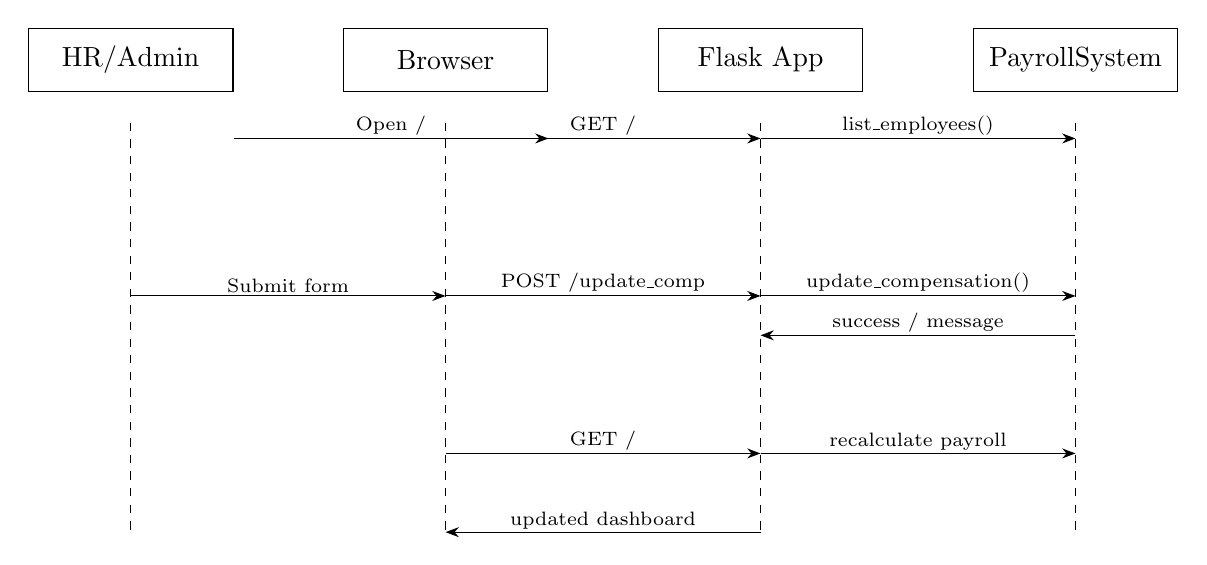
\begin{tikzpicture}[
        lifeline/.style={draw, rectangle, minimum width=2.6cm, minimum height=0.8cm, align=center},
        msg/.style={-Stealth},
        lab/.style={font=\scriptsize, inner sep=1pt}
    ]
        % Lifelines (top boxes)
        \node[lifeline] (hr) at (0,0) {HR/Admin};
        \node[lifeline] (br) at (4,0) {Browser};
        \node[lifeline] (fa) at (8,0) {Flask App};
        \node[lifeline] (ps) at (12,0) {PayrollSystem};

        % Dashed lifelines
        \draw[dashed] (0,-0.8) -- (0,-6);
        \draw[dashed] (4,-0.8) -- (4,-6);
        \draw[dashed] (8,-0.8) -- (8,-6);
        \draw[dashed] (12,-0.8) -- (12,-6);

        % --- Phase 1: Initial dashboard load (y = -1) ---
        \draw[msg] (hr.east) ++(0,-1) -- node[lab,above]{Open /} ++(4,0);
        \draw[msg] (4,-1) -- node[lab,above]{GET /} (8,-1);
        \draw[msg] (8,-1) -- node[lab,above]{list\_employees()} (12,-1);

        % --- Phase 2: Submit update form (y = -3) ---
        \draw[msg] (0,-3) -- node[lab,above]{Submit form} (4,-3);
        \draw[msg] (4,-3) -- node[lab,above]{POST /update\_comp} (8,-3);
        \draw[msg] (8,-3) -- node[lab,above]{update\_compensation()} (12,-3);
        \draw[msg] (12,-3.5) -- node[lab,above]{success / message} (8,-3.5);

        % --- Phase 3: Reload dashboard (y = -5) ---
        \draw[msg] (4,-5) -- node[lab,above]{GET /} (8,-5);
        \draw[msg] (8,-5) -- node[lab,above]{recalculate payroll} (12,-5);
        \draw[msg] (8,-6) -- node[lab,above]{updated dashboard} (4,-6);
    \end{tikzpicture}
    \caption{Sequence Diagram for Updating Compensation and Viewing Payroll}
\end{figure}

\clearpage

\section{Implementation Overview}
This section summarizes how the requirements of the Payroll Management System were realized in the implemented codebase.

\subsection{Technology Stack}
The application is implemented in Python using the Flask micro–web framework. 
Server-side logic resides primarily in the \texttt{payroll.py} module (business logic) and \texttt{app.py} (HTTP routes and request handling). 
The user interface is rendered using a single Jinja2 HTML template (\texttt{templates/index.html}) styled with responsive CSS, while data is persisted locally in a JSON file (\texttt{payroll\_data.json}).

\subsection{Key Modules and Responsibilities}
\textbf{PayrollSystem (payroll.py).} Encapsulates all core domain logic: employee management, compensation updates, overtime-aware payroll calculations, summary statistics, and CSV export of payroll data. 
It is responsible for loading and saving the JSON data file, validating inputs (e.g., non-negative hours, allowances, and deductions), and returning structured breakdowns of gross and net pay.

\noindent\textbf{Flask Application (app.py).} Exposes HTTP endpoints for the main dashboard, adding and removing employees, updating compensation, and downloading the CSV report. 
Each route coordinates form input validation, delegates work to the \texttt{PayrollSystem} instance, and uses flash messages to provide immediate feedback to the user.

\noindent\textbf{Presentation Layer (index.html).} Implements a single-page layout with sections for employee management, compensation updates, payroll tables, and summary cards. 
Server-provided data (employees, payroll rows, and summary totals) are dynamically injected through Jinja2 template variables to keep the view logic minimal and maintainable.

\subsection{Data Flow}
When the application starts, \texttt{PayrollSystem.loadData()} reads existing records from \texttt{payroll\_data.json}. 
User actions sent via forms (add/update/remove) are handled by Flask routes, which call the appropriate \texttt{PayrollSystem} methods; these methods mutate the in-memory employee dictionary and immediately persist changes back to JSON. 
For each page load, the dashboard route queries the current employees, detailed payroll, and summary statistics, which are then rendered into HTML for the browser.

\subsection{Extensibility Considerations}
The codebase separates routing, business logic, and presentation concerns to support future extension. 
For larger deployments, the JSON persistence layer could be replaced with a relational database without changing the Flask views, and additional features such as authentication, role-based access, or more sophisticated tax and deduction rules can be added by extending the \texttt{PayrollSystem} class and UI forms.

\clearpage

\section{Testing \& Test Cases}
This section documents the key functional and negative test cases executed on the Payroll Management System, along with their expected and actual outcomes.

\subsection{Functional Test Cases}
\begin{center}
\begin{tabular}{|p{1.2cm}|p{4.3cm}|p{4.5cm}|p{3cm}|}
\hline
\textbf{ID} & \textbf{Description} & \textbf{Expected Result} & \textbf{Actual Result} \\
\hline
FT1 & Add a new employee with valid name, ID, department, hourly rate, allowances, and deductions. 
     & Employee appears in the Employees table, data is written to \texttt{payroll\_data.json}, and a success flash message is shown. 
     & As expected. Employee persisted and visible on dashboard reload. \\
\hline
FT2 & Update compensation (hours, allowances, deductions) for an existing employee via the Update Compensation form. 
     & Employee row reflects new values; payroll and summary totals update accordingly without errors. 
     & As expected. Payroll cards and totals recomputed correctly. \\
\hline
FT3 & Remove an existing employee using the Remove button. 
     & Employee disappears from the Employees and Payroll tables; totals decrease by that employee's pay. 
     & As expected. JSON data file updated and UI refreshed. \\
\hline
FT4 & Generate payroll with multiple employees, including some with overtime hours (\(> 40\)). 
     & Regular and overtime hours computed correctly; gross and net totals match manual calculations. 
     & As expected. Verified against hand-calculated examples. \\
\hline
FT5 & Download the CSV payroll report from the dashboard. 
     & Browser downloads a CSV file containing one row per employee plus aggregated totals; values match those shown on screen. 
     & As expected. File opens correctly in spreadsheet software with consistent data. \\
\hline
FT6 & Refresh the dashboard after restarting the Flask server. 
     & Previously added employees and their hours/compensation values are reloaded from \texttt{payroll\_data.json} without loss. 
     & As expected. All records reappear and totals match the state before restart. \\
\hline
FT7 & Leave allowances and deductions blank in the Update Compensation form while changing only hours. 
     & Only the hours field is updated; existing allowances and deductions remain unchanged. 
     & As expected. JSON data shows only hours modified and payroll totals update accordingly. \\
\hline
\end{tabular}
\end{center}

\subsection{Negative Test Cases}
\begin{center}
\begin{tabular}{|p{1.2cm}|p{4.3cm}|p{4.5cm}|p{3cm}|}
\hline
\textbf{ID} & \textbf{Description} & \textbf{Expected Result} & \textbf{Actual Result} \\
\hline
NT1 & Attempt to add an employee with a duplicate Employee ID. 
     & System rejects the request, shows an error flash message, and leaves existing data unchanged. 
     & As expected. No duplicate created; original record preserved. \\
\hline
NT2 & Enter negative hours or deductions/allowances in the Update Compensation form. 
     & Validation fails; user sees a clear error message and values are not saved to the JSON file. 
     & As expected. Input rejected and previous values remain intact. \\
\hline
NT3 & Request removal of a non-existent employee ID via the Remove button URL. 
     & System shows an error flash message (“Employee not found”) and makes no changes to stored data. 
     & As expected. No records deleted and payroll totals remain unchanged. \\
\hline
NT4 & Submit the Add Employee form with a non-numeric hourly rate (e.g., letters). 
     & Form handling catches the conversion error and displays a validation message without creating any employee record. 
     & As expected. No new employee appears and JSON file is unchanged. \\
\hline
\end{tabular}
\end{center}

\clearpage

\section{Results / Screenshots}
This section presents visual evidence of the working Payroll Management System. 
Space is reserved below for key screenshots demonstrating the main flows.

\subsection*{Dashboard and Summary View}
Overview of the main dashboard showing employee list, payroll table, and summary cards.

\begin{figure}[h!]
    \centering
    % Replace "images/dashboard.png" with the actual path to your screenshot
    \includegraphics[width=\textwidth]{1.png}
    
     \includegraphics[width=\textwidth]{2.png}
    \caption{Dashboard and Summary View}
\end{figure}

\subsection*{Employee Management}
Screenshots showing adding a new employee, updating compensation, and removing an employee.

\begin{figure}[h!]
    \centering
   \includegraphics[width=\textwidth]{5.png}
    \includegraphics[width=\textwidth]{7.png}
    \caption{Employee Management Screens}
\end{figure}

\subsection*{Reporting and Export}
Screenshots for the CSV export confirmation/download and example of the opened CSV in a spreadsheet.

\begin{figure}[h!]
    \centering
    % Replace "images/reporting_export.png" with the actual path to your screenshot
    \includegraphics[width=\textwidth]{3.png}
    \includegraphics[width=\textwidth]{4.png}
    \includegraphics[width=\textwidth]{6.png}
    \caption{Reporting and CSV Export}
\end{figure}

\clearpage

\section{Conclusion}
The enhanced Payroll Management System successfully meets the functional and non-functional requirements outlined in the SRS. 
It provides a clean single-page interface for managing employees, tracking hours, handling overtime, and applying allowances and deductions while persisting data reliably in JSON. 
Additional features such as CSV export, dashboard summaries, and validation-driven error handling make the solution suitable for academic projects and small organizations needing lightweight payroll support. 
The modular structure of the codebase allows future teams to extend the system with stronger security, database integration, and more complex payroll rules.

\section{References}
\begin{itemize}
    \item Python Software Foundation. \textit{Python 3.x Documentation}. Available at: \url{https://docs.python.org/3/}
    \item Pallets Projects. \textit{Flask Web Framework Documentation}. Available at: \url{https://flask.palletsprojects.com/}
    \item Overleaf. \textit{LaTeX Documentation and Templates}. Available at: \url{https://www.overleaf.com/learn}
    \item W3C. \textit{HTML5 and CSS Specifications}. Available at: \url{https://www.w3.org/}
\end{itemize}

\end{document}